\documentclass[12pt,a4paper]{article}
\usepackage[utf8]{vietnam}
\usepackage{amsmath,amssymb}
\usepackage{geometry}
\geometry{top=1.5cm,bottom=1.2cm,left=1.4cm,right=1.4cm,headheight=28pt,headsep=12pt,footskip=18pt}
\usepackage{tikz}
\usepackage{xcolor}
\usepackage{enumerate}
\usepackage{graphicx}
\usepackage[version=4]{mhchem}
\usepackage{fancyhdr}
\usepackage{ex_test}

\renewcommand{\baselinestretch}{0.96}
\setlength{\parskip}{0pt}

\definecolor{hfRed}{RGB}{211,47,47}
\definecolor{hfGreen}{RGB}{139,195,144}

\providecommand{\False}{}

\pagestyle{fancy}
\fancyhf{}
\fancyhead[L]{\small\itshape\color{hfRed} Tài liệu lưu hành nội bộ}
\fancyhead[R]{\small\itshape\color{hfRed} Thầy \textbf{TRẦN VĂN THẠNH} - 0777.470.803}
\renewcommand{\headrulewidth}{0.8pt}
\renewcommand{\headrule}{\hbox to\headwidth{\color{hfGreen}\leaders\hrule height \headrulewidth\hfill}}

\fancyfoot[L]{\small\itshape\color{hfRed} CS1: 6/15 Nguyễn Hoàng, P. Kim Long, TP Huế \quad|\quad CS2: 24 Đặng Thái Thân, TP Huế}
\fancyfoot[R]{\small\bfseries\color{hfRed} Trang \thepage}
\renewcommand{\footrulewidth}{0.8pt}
\renewcommand{\footrule}{\hbox to\headwidth{\color{hfGreen}\leaders\hrule height \footrulewidth\hfill}}

\fancypagestyle{firstpage}{
  \fancyhf{}
  \renewcommand{\headrulewidth}{0pt}
  \fancyfoot[L]{\small\itshape\color{hfRed} CS1: 6/15 Nguyễn Hoàng, P. Kim Long, TP Huế \quad|\quad CS2: 24 Đặng Thái Thân, TP Huế}
  \fancyfoot[R]{\small\bfseries\color{hfRed} Trang \thepage}
  \renewcommand{\footrulewidth}{0.8pt}
  \renewcommand{\footrule}{\hbox to\headwidth{\color{hfGreen}\leaders\hrule height \footrulewidth\hfill}}
}

\begin{document}
\thispagestyle{firstpage}

\noindent
\begin{minipage}[t]{0.44\textwidth}
	\centering\fontsize{10pt}{12pt}\selectfont
	\textbf{SỞ GIÁO DỤC VÀ ĐÀO TẠO THỪA THIÊN HUẾ}\\
	\textbf{ĐỀ CHÍNH THỨC}\\
	\textit{(Đề thi có 04 trang)}
\end{minipage}\hfill
\begin{minipage}[t]{0.54\textwidth}
	\centering\small
	\textbf{ĐỀ KIỂM TRA ĐỊNH KỲ CHƯƠNG 1 (ESTER -- LIPID)}\\
	\textbf{MÔN: HOÁ HỌC -- LỚP 12}\\
	\textit{Thời gian làm bài: 50 phút (không kể thời gian phát đề)}\\
	\fbox{\textbf{MÃ ĐỀ: 103}}
\end{minipage}

\smallskip
\begin{center}
	{\color{hfRed}\textbf{\large (BẢN GIÁO VIÊN -- CÓ LỜI GIẢI CHI TIẾT)}}
\end{center}

\smallskip
\noindent\hrulefill
\smallskip

\noindent\textbf{Họ, tên thí sinh:} \dotfill\ \textbf{Lớp:} \dotfill\ \textbf{Số báo danh:} \dotfill

\smallskip
\noindent\textit{(Cho biết nguyên tử khối: H = 1; C = 12; N = 14; O = 16; Na = 23; K = 39; Br = 80; Cl = 35,5).}
\smallskip

\noindent
\textbf{PHẦN I (4,5 điểm -- 18 câu): Câu trắc nghiệm nhiều phương án lựa chọn.}\\
\textit{Thí sinh trả lời từ câu 1 đến câu 18. Mỗi câu hỏi thí sinh chỉ chọn một phương án.}

\Opensolutionfile{ans}[ans-de03gv]

\begin{ex}
(SBT - KNTT). Chất nào sau đây thuộc loại ester?
\choice
{\True $\ce{HCOOCH3}$}
{$\ce{CH3COOH}$}
{$\ce{HCOOH}$}
{$\ce{CH3COCH3}$}
\loigiai{
$\ce{HCOOCH3}$ (methyl formate) là ester tạo từ formic acid và methanol.\\
$\ce{CH3COOH}$ và $\ce{HCOOH}$ là carboxylic acid; $\ce{CH3COCH3}$ là ketone.\\
\textbf{Chọn A.}}
\end{ex}

\begin{ex}
(SBT - KNTT, CTST). Số đồng phân cấu tạo của ester có công thức $\ce{C4H8O2}$ là
\choice
{2}
{3}
{\True 4}
{5}
\loigiai{
Các đồng phân cấu tạo ester $\ce{C4H8O2}$:\\
(1) $\ce{HCOOCH2CH2CH3}$; (2) $\ce{HCOOCH(CH3)2}$; (3) $\ce{CH3COOCH2CH3}$; (4) $\ce{CH3CH2COOCH3}$.\\
$\Rightarrow$ Có 4 đồng phân cấu tạo.\\
\textbf{Chọn C.}}
\end{ex}

\begin{ex}
(SBT - KNTT). Ethyl propanoate là ester tạo nên mùi thơm đặc trưng của quả dứa. Công thức của ethyl propanoate là
\choice
{$\ce{CH3COOC2H5}$}
{$\ce{C2H5COOCH2CH2CH3}$}
{$\ce{CH3COOCH2CH2CH3}$}
{\True $\ce{C2H5COOC2H5}$}
\loigiai{
Ethyl propanoate tạo bởi propanoic acid ($\ce{C2H5COOH}$) và ethanol ($\ce{C2H5OH}$), công thức là $\ce{C2H5COOC2H5}$.\\
\textbf{Chọn D.}}
\end{ex}

\begin{ex}
Ester nào sau đây tác dụng với dung dịch $\ce{NaOH}$ thu được sodium formate?
\choice
{$\ce{C2H5COOC2H5}$}
{$\ce{CH3COOC2H5}$}
{$\ce{CH3COOCH3}$}
{\True $\ce{HCOOCH3}$}
\loigiai{
Sodium formate là $\ce{HCOONa}$. Phản ứng: $\ce{HCOOCH3 + NaOH -> HCOONa + CH3OH}$.\\
\textbf{Chọn D.}}
\end{ex}

\begin{ex}
Khi đun nóng chất X có công thức phân tử $\ce{C3H6O2}$ với dung dịch $\ce{NaOH}$ thu được $\ce{CH3COONa}$. Công thức cấu tạo của X là
\choice
{$\ce{CH3COOC2H5}$}
{$\ce{HCOOC2H5}$}
{\True $\ce{CH3COOCH3}$}
{$\ce{C2H5COOH}$}
\loigiai{
X là $\ce{C3H6O2}$ tạo $\ce{CH3COONa}$ nên X là ester của acetic acid: $\ce{CH3COOCH3}$ (methyl acetate).\\
\textbf{Chọn C.}}
\end{ex}

\begin{ex}
Chất nào sau đây phản ứng với dung dịch $\ce{NaOH}$ tạo thành $\ce{HCOONa}$ và $\ce{C2H5OH}$?
\choice
{\True $\ce{HCOOC2H5}$}
{$\ce{CH3COOC2H5}$}
{$\ce{CH3COOCH3}$}
{$\ce{HCOOCH3}$}
\loigiai{
Phản ứng: $\ce{HCOOC2H5 + NaOH -> HCOONa + C2H5OH}$.\\
\textbf{Chọn A.}}
\end{ex}

\begin{ex}
(SBT - CTST). Tính chất nào sau đây không phải là tính chất thích hợp giúp ethyl methanoate ($\ce{HCOOC2H5}$) được sử dụng trong sản xuất một số loại nước hoa?
\choice
{\True Khả năng dễ cháy}
{Có mùi thơm dễ chịu}
{Không độc hại}
{Nhiệt độ sôi thấp}
\loigiai{
Ethyl methanoate được dùng trong nước hoa vì có mùi thơm, không độc và dễ bay hơi (nhiệt độ sôi thấp). Khả năng dễ cháy là nhược điểm về an toàn phòng cháy chữa cháy.\\
\textbf{Chọn A.}}
\end{ex}

\begin{ex}
Nguyên liệu nào sau đây là nguyên liệu vô cơ chủ yếu trong phản ứng xà phòng hoá?
\choice
{Calcium hydroxide $\ce{Ca(OH)2}$}
{\True Sodium hydroxide $\ce{NaOH}$}
{Barium hydroxide $\ce{Ba(OH)2}$}
{Iron(III) hydroxide $\ce{Fe(OH)3}$}
\loigiai{
Trong công nghiệp sản xuất xà phòng, người ta thường dùng base kiềm vô cơ là $\ce{NaOH}$ hoặc $\ce{KOH}$.\\
\textbf{Chọn B.}}
\end{ex}

\begin{ex}
Xà phòng được tổng hợp theo phản ứng:
\begin{center}
	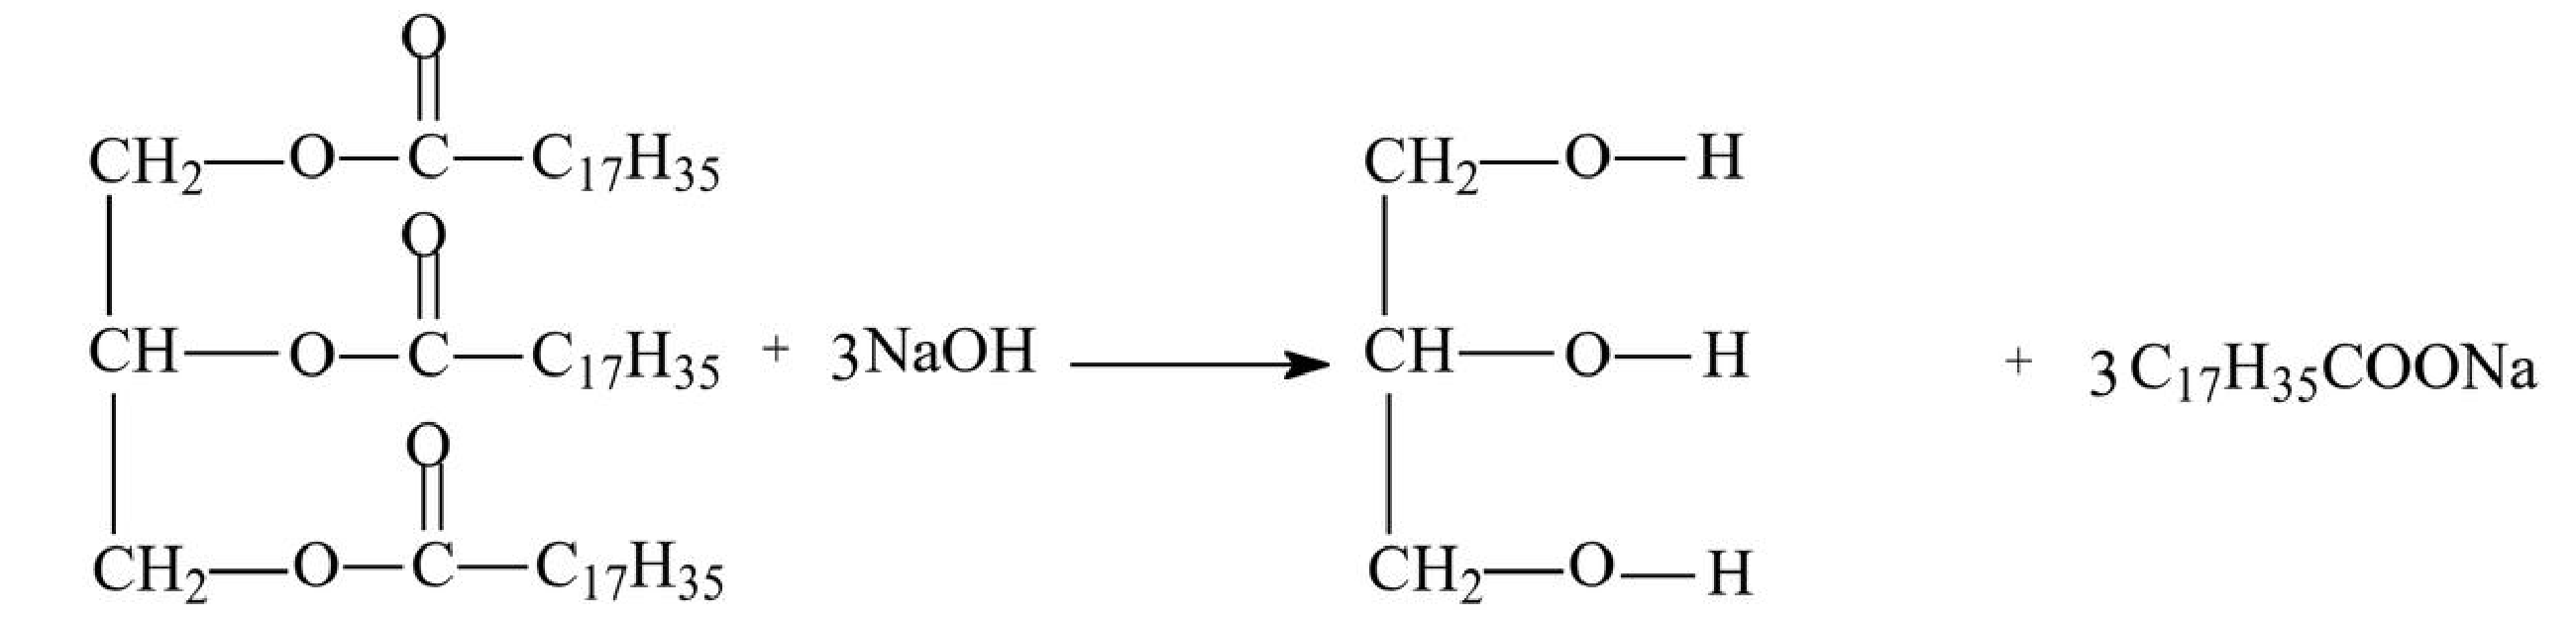
\includegraphics[width=12cm]{images_crop_de03/cau9_phan_ung_xa_phong_hoa.png}
\end{center}
Phản ứng trên là ví dụ của
\choice
{phản ứng ngưng tụ}
{phản ứng ester hóa}
{phản ứng oxi hóa}
{\True phản ứng thủy phân}
\loigiai{
Đây là phản ứng thuỷ phân chất béo trong môi trường kiềm (phản ứng xà phòng hoá).\\
\textbf{Chọn D.}}
\end{ex}

\begin{ex}
Phát biểu nào sau đây không đúng?
\choice
{Chất béo không tan trong nước, nhẹ hơn nước nhưng tan nhiều trong dung môi hữu cơ}
{\True Dầu ăn và mỡ bôi trơn có cùng thành phần nguyên tố}
{Chất béo là triester của glycerol với các monocarboxylic acid có số chẵn nguyên tử carbon (12 - 24), mạch carbon dài, không phân nhánh}
{Phản ứng thủy phân chất béo trong môi trường base là phản ứng một chiều}
\loigiai{
Dầu ăn là chất béo (chứa C, H, O), còn mỡ bôi trơn máy móc là hỗn hợp các hydrocarbon (chỉ chứa C, H). Do đó thành phần nguyên tố của chúng khác nhau.\\
\textbf{Chọn B.}}
\end{ex}

\begin{ex}
Nguyên nhân nào làm cho bồ kết có khả năng giặt rửa:
\choice
{\True Vì bồ kết có những chất có cấu tạo kiểu đầu phân cực gắn với đuôi không phân cực}
{Vì bồ kết có thành phần là este của glycerine}
{Vì trong bồ kết có những chất oxi hóa mạnh}
{Vì trong bồ kết có chất khử mạnh}
\loigiai{
Quả bồ kết chứa hoạt chất saponin (chất hoạt động bề mặt) có cấu tạo gồm đầu phân cực (ưa nước) gắn với đuôi không phân cực (kị nước/ưa dầu) giúp nhũ hoá và giặt rửa.\\
\textbf{Chọn A.}}
\end{ex}

\begin{ex}
Cho phản ứng ester hóa: $\ce{RCOOH + R^{\prime}OH <=>[\ce{H2SO4},\, t^\circ] RCOOR^{\prime} + H2O}$. Để phản ứng chuyển dịch ưu tiên theo chiều thuận người ta thường:
\choice
{Dùng $\ce{H2SO4}$ đặc để hút nước và làm xúc tác}
{Chưng cất để tách ester ra khỏi hỗn hợp phản ứng}
{Tăng nồng độ của acid hoặc alcohol}
{\True Tất cả đều đúng}
\loigiai{
Theo nguyên lí Le Chatelier, việc hút nước, tách ester khỏi phản ứng hoặc tăng nồng độ chất phản ứng đều làm cân bằng chuyển dịch theo chiều thuận.\\
\textbf{Chọn D.}}
\end{ex}

\begin{ex}
(SBT-CD). Phát biểu nào sau đây là không đúng?
\choice
{So với các đồng phân là carboxylic acid, ester luôn có nhiệt độ sôi thấp hơn}
{Phản ứng ester hoá là phản ứng thuận nghịch}
{\True Phản ứng xà phòng hoá là phản ứng thuận nghịch}
{Ester là những chất lỏng hoặc chất rắn ở nhiệt độ thường}
\loigiai{
Phản ứng xà phòng hoá là phản ứng một chiều (không thuận nghịch) vì anion carboxylate tạo thành không phản ứng lại với alcohol.\\
\textbf{Chọn C.}}
\end{ex}

\begin{ex}
Thủy phân ester có công thức $\ce{C4H8O2}$ (với xúc tác acid), thu được hai sản phẩm hữu cơ X và Y. Từ X có thể điều chế trực tiếp ra Y. Vậy chất X là:
\choice
{Methyl alcohol}
{Ethyl acetate}
{Formic acid}
{\True Ethyl alcohol}
\loigiai{
$\ce{CH3COOC2H5 + H2O <=>[\ce{H+}, t^\circ] CH3COOH (Y) + C2H5OH (X)}$.\\
Lên men giấm: $\ce{C2H5OH + O2 ->[\text{men giấm}] CH3COOH + H2O}$. Vậy X là ethyl alcohol.\\
\textbf{Chọn D.}}
\end{ex}

\begin{ex}
(SBT-CD). Thuỷ phân ester E có công thức phân tử $\ce{C4H8O2}$ với xúc tác acid vô cơ loãng, thu được hai sản phẩm hữu cơ X, Y (chỉ chứa các nguyên tử C, H, O). Từ X có thể điều chế trực tiếp ra Y bằng một phản ứng duy nhất. Chất X là chất nào sau đây?
\choice
{Acetic acid}
{\True Ethyl alcohol}
{Ethyl acetate}
{Formic acid}
\loigiai{
Tương tự, ester E là $\ce{CH3COOC2H5}$. X là $\ce{C2H5OH}$ (ethyl alcohol) và Y là $\ce{CH3COOH}$.\\
\textbf{Chọn B.}}
\end{ex}

\begin{ex}
(SGK - KNTT). Cho các phát biểu sau:\\
(1) Một số ester có mùi thơm nên được dùng làm chất tạo hương trong công nghiệp thực phẩm và mĩ phẩm.\\
(2) Chất béo là triester của glycerol với acid béo.\\
(3) Chất béo tan tốt trong nước.\\
(4) Mỡ động vật, dầu thực vật có thể được dùng làm nguyên liệu để sản xuất xà phòng.\\
(5) Phản ứng thuỷ phân ester trong môi trường acid luôn là phản ứng một chiều.\\
Số phát biểu đúng là
\choice
{2}
{\True 3}
{4}
{5}
\loigiai{
Các phát biểu đúng gồm: (1), (2), (4). (3) sai vì chất béo không tan trong nước; (5) sai vì thuỷ phân ester trong môi trường acid là phản ứng thuận nghịch.\\
\textbf{Chọn B.}}
\end{ex}

\begin{ex}
(SBT-CD). Tiến hành thí nghiệm điều chế isoamyl acetate (chất có mùi chuối chín) theo thứ tự các bước sau đây:\\
Bước 1: Cho khoảng $3\text{ mL}$ $\ce{CH3CH(CH3)CH2CH2OH}$, $3\text{ mL}$ $\ce{CH3COOH}$ và vài giọt $\ce{H2SO4}$ đặc vào ống nghiệm.\\
Bước 2: Lắc đều ống nghiệm rồi đun cách thuỷ (trong nồi nước nóng) khoảng 5--7 phút ở $65-70^\circ\text{C}$.\\
Bước 3: Làm lạnh, sau đó thêm khoảng $5\text{ mL}$ dung dịch $\ce{NaCl}$ bão hoà vào ống nghiệm.\\
Cho các phát biểu sau:\\
(a) $\ce{H2SO4}$ đặc có vai trò xúc tác cho phản ứng tạo isoamyl acetate.\\
(b) Thêm dung dịch $\ce{NaCl}$ bão hoà vào để tránh phân huỷ sản phẩm.\\
(c) Sau bước 2, trong ống nghiệm vẫn còn $\ce{CH3CH(CH3)CH2CH2OH}$ và $\ce{CH3COOH}$.\\
(d) Sau bước 3, trong ống nghiệm thu được hỗn hợp chất lỏng đồng nhất.\\
Số phát biểu đúng là
\choice
{4}
{5}
{3}
{\True 2}
\loigiai{
(a) Đúng: $\ce{H2SO4}$ đặc làm chất xúc tác và hút nước.\\
(b) Sai: Thêm $\ce{NaCl}$ bão hoà nhằm tăng khối lượng riêng dung dịch và giảm độ tan của ester để ester tách lớp.\\
(c) Đúng: Phản ứng thuận nghịch nên các chất tham gia vẫn còn.\\
(d) Sai: Sau bước 3 ester tách lớp nổi lên trên, không đồng nhất.\\
$\Rightarrow$ Có 2 phát biểu đúng: (a), (c).\\
\textbf{Chọn D.}}
\end{ex}

\begin{ex}
Một loại chất béo có chứa 65\% tripalmitin về khối lượng. Để sản xuất 3 triệu hộp kem dưỡng da (có chứa chất dưỡng ẩm glycerol) cần dùng tối thiểu $x\text{ tấn}$ loại chất béo trên cho phản ứng với dung dịch $\ce{NaOH}$, đun nóng. Biết hiệu suất phản ứng đạt 80\%. Biết rằng trong mỗi hộp kem dưỡng da có chứa $5\text{ gam}$ glycerol. Giá trị của $x$ là
\choice
{152{,}7}
{525{,}4}
{\True 252{,}7}
{175{,}7}
\loigiai{
- $m_{\text{glycerol}} = 3 \times 10^6 \times 5\text{ g} = 15 \times 10^6\text{ g} = 15\text{ tấn}$.\\
- $\ce{(C15H31COO)3C3H5 + 3NaOH -> 3C15H31COONa + C3H5(OH)3}$.\\
$m_{\text{tripalmitin (LT)}} = 15 \times \dfrac{806}{92} \approx 131{,}413\text{ tấn}$.\\
- Vì $H = 80\% \Rightarrow m_{\text{tripalmitin (TT)}} = \dfrac{131{,}413}{0{,}8} = 164{,}266\text{ tấn}$.\\
- Vì chất béo chứa 65\% tripalmitin $\Rightarrow x = \dfrac{164{,}266}{0{,}65} \approx \mathbf{252{,}7\text{ tấn}}$.\\
\textbf{Chọn C.}}
\end{ex}

\Closesolutionfile{ans}

\vspace{0.3cm}
\noindent
\textbf{PHẦN II (4,0 điểm -- 4 câu): Câu trắc nghiệm đúng sai.}\\
\textit{Thí sinh trả lời từ câu 1 đến câu 4. Trong mỗi ý a), b), c), d) ở mỗi câu, thí sinh chọn đúng hoặc sai.}

\setcounter{ex}{0}

\begin{ex}
Nhiều loại bơ thực vật (chất béo no ở dạng rắn) được tạo ra bởi quá trình hydrogen hóa một phần dầu thực vật (chất béo không no ở dạng lỏng).
\begin{center}
	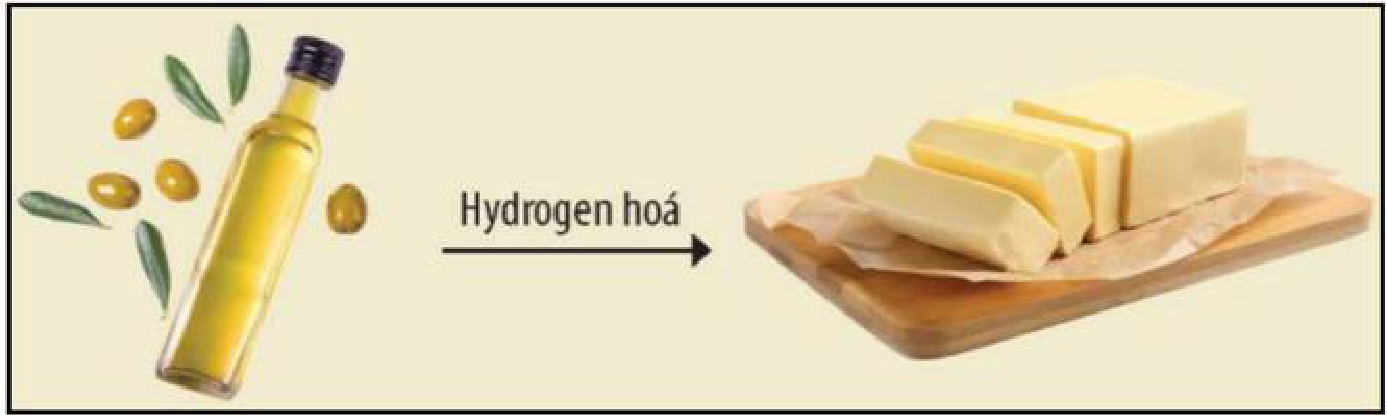
\includegraphics[width=9.5cm]{images_crop_de03/cau1_hydrogen_hoa_dau_an.png}
\end{center}
\choiceTF[t]
{\False Trong công nghiệp, người ta sử dụng phản ứng này để chuyển hóa chất béo lỏng thành chất béo rắn và ngược lại.}
{\True 1 mol triolein (chất béo dạng lỏng) phản ứng tối đa với 3 mol $\ce{H2}$ (Ni, $t^\circ$) tạo thành tristearin (chất béo dạng rắn).}
{\True Do chứa các liên kết đôi ($\ce{C=C}$) trong phân tử, nên chất béo không no bị oxi hóa chậm bởi oxygen trong không khí tạo ra các chất có mùi khó chịu, làm cho dầu mỡ bị ôi.}
{\False Số nguyên tử carbon ở chất béo lỏng và rắn khác nhau.}
\loigiai{
\begin{itemize}
	\item a) \textbf{Sai.} Phản ứng hydrogen hoá chỉ dùng để chuyển chất béo lỏng thành chất béo rắn; không có chiều ngược lại.
	\item b) \textbf{Đúng.} $\ce{(C17H33COO)3C3H5 + 3H2 ->[Ni, t^\circ] (C17H35COO)3C3H5}$.
	\item c) \textbf{Đúng.} Liên kết $\ce{C=C}$ bị oxi hóa chậm bởi $\ce{O2}$ không khí tạo các hợp chất peroxide rồi phân huỷ thành aldehyde/ketone có mùi ôi.
	\item d) \textbf{Sai.} Cả triolein và tristearin đều có cùng số nguyên tử carbon ($57\text{ C}$).
\end{itemize}}
\end{ex}

\begin{ex}
Aspirin được sử dụng làm thuốc giảm đau, hạ sốt. Sau khi uống, aspirin bị thuỷ phân trong cơ thể tạo thành salicylic acid. Salicylic acid ức chế quá trình sinh tổng hợp prostaglandin (chất gây đau, sốt và viêm khi nồng độ trong máu cao hơn mức bình thường).
\begin{center}
	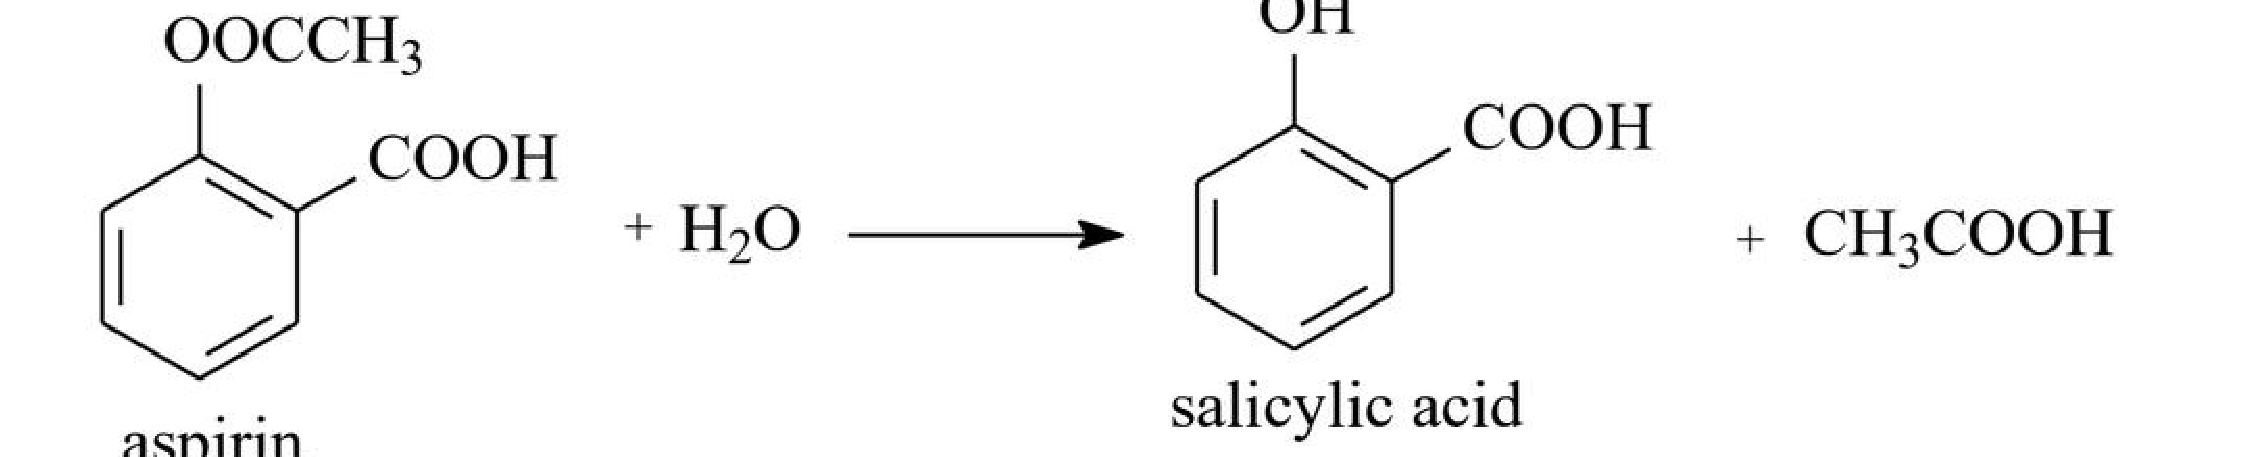
\includegraphics[width=11cm]{images_crop_de03/cau2_thuy_phan_aspirin.png}
\end{center}
\choiceTF[t]
{\True Aspirin có công thức phân tử $\ce{C9H8O4}$.}
{\True Salicylic acid có công thức phân tử $\ce{C7H6O3}$.}
{\False Aspirin có độ bất bão hòa $k = 5$.}
{\False Salicylic acid là hợp chất hữu cơ đa chức.}
\loigiai{
\begin{itemize}
	\item a) \textbf{Đúng.} Aspirin ($\ce{CH3COOC6H4COOH}$) có CTPT là $\ce{C9H8O4}$.
	\item b) \textbf{Đúng.} Salicylic acid ($\ce{HOC6H4COOH}$) có CTPT là $\ce{C7H6O3}$.
	\item c) \textbf{Sai.} $k = \dfrac{2 \times 9 + 2 - 8}{2} = 6$ (1 vòng benzen $k=4$, 1 nhóm $-\ce{COOH}$ $k=1$, 1 nhóm ester $k=1$).
	\item d) \textbf{Sai.} Salicylic acid chứa đồng thời nhóm $-\ce{OH}$ phenol và $-\ce{COOH}$ nên là hợp chất \textbf{tạp chức}.
\end{itemize}}
\end{ex}

\begin{ex}
(SBT - CTST). Cho các chất sau:
\begin{center}
	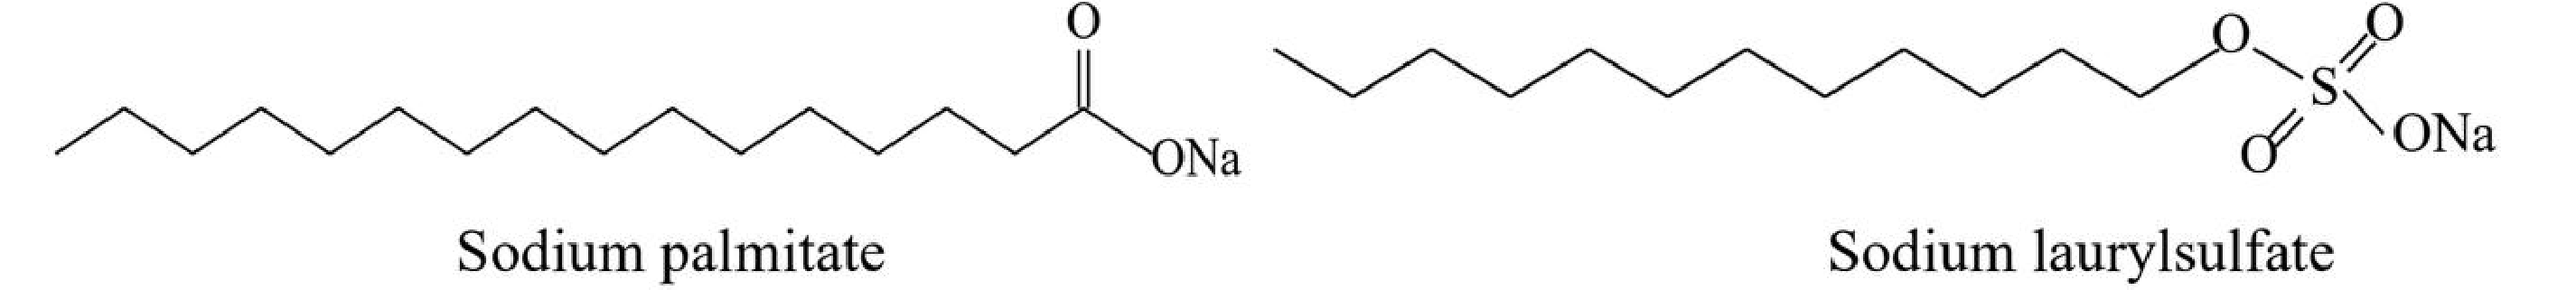
\includegraphics[width=12cm]{images_crop_de03/cau3_sodium_palmitate_laurylsulfate.png}
\end{center}
Xét tính đúng/sai của các phát biểu sau:
\choiceTF[t]
{\False Sodium palmitate và sodium laurylsulfate đều là thành phần chính của xà phòng.}
{\True Sodium palmitate và sodium laurylsulfate đều có tính năng giặt rửa.}
{\False Sodium palmitate và sodium laurylsulfate đều tạo muối khó tan trong nước cứng.}
{\True Sodium palmitate và sodium laurylsulfate đều có đầu ưa nước gắn với đuôi kị nước.}
\loigiai{
\begin{itemize}
	\item a) \textbf{Sai.} Sodium palmitate là thành phần xà phòng; sodium laurylsulfate là thành phần chất giặt rửa tổng hợp.
	\item b) \textbf{Đúng.} Cả hai đều có tính hoạt động bề mặt và tính năng giặt rửa.
	\item c) \textbf{Sai.} Chất giặt rửa tổng hợp (sodium laurylsulfate) không tạo muối khó tan trong nước cứng.
	\item d) \textbf{Đúng.} Cả hai đều có đầu ưa nước mang điện tích và đuôi hydrocarbon dài kị nước.
\end{itemize}}
\end{ex}

\begin{ex}
Các chất béo có thể là chất lỏng hoặc rắn, có trong một số loại động thực vật.
\choiceTF[t]
{\False Tripalmitin là một loại chất béo không no có trong mỡ động vật và dầu cọ có công thức phân tử là $\ce{C51H98O6}$.}
{\True Tristearin thu được từ mỡ động vật là một sản phẩm phụ của chế biến thịt bò có công thức phân tử là $\ce{C57H110O6}$.}
{\True Triolein chiếm 4-30\% trong dầu oliu là chất béo không no ở trạng thái lỏng có công thức là $\ce{C57H104O6}$.}
{\False Glyceryl trilinoleate hay trilinolein là chất béo no ở trạng thái rắn có công thức phân tử là $\ce{C57H98O6}$.}
\loigiai{
\begin{itemize}
	\item a) \textbf{Sai.} Tripalmitin $\ce{(C15H31COO)3C3H5}$ là chất béo \textbf{no}.
	\item b) \textbf{Đúng.} Tristearin có công thức $\ce{C57H110O6}$, là chất béo no thể rắn.
	\item c) \textbf{Đúng.} Triolein có công thức $\ce{C57H104O6}$, chứa 3 liên kết đôi $\ce{C=C}$ nên là chất béo không no ở thể lỏng.
	\item d) \textbf{Sai.} Trilinolein $\ce{(C17H31COO)3C3H5}$ chứa các gốc linoleic acid không no nên là chất béo \textbf{không no}.
\end{itemize}}
\end{ex}

\vspace{0.3cm}
\noindent
\textbf{PHẦN III (1,5 điểm -- 6 câu): Câu trắc nghiệm yêu cầu trả lời ngắn.}\\
\textit{Thí sinh trả lời từ câu 1 đến câu 6. Mỗi câu hỏi thí sinh điền câu trả lời ngắn gọn theo yêu cầu.}

\setcounter{ex}{0}

\begin{ex}
(SBT - CTST). Có bao nhiêu ester của methyl alcohol có công thức phân tử là $\ce{C5H10O2}$?
\loigiai{
Ester có dạng $\ce{RCOOCH3}$. Gốc $\ce{R-}$ có 3 C gồm propyl và isopropyl: $\ce{CH3CH2CH2COOCH3}$ và $\ce{(CH3)2CHCOOCH3}$.\\
$\Rightarrow$ Có \textbf{2} ester thoả mãn.\\
\textbf{Đáp số: 2.}}
\end{ex}

\begin{ex}
(SBT - CTST). Có bao nhiêu triglyceride mà khi xà phòng hoá hoàn toàn thu được glycerol cùng hỗn hợp chỉ gồm muối của palmitic acid và stearic acid?
\loigiai{
Chứa cả 2 gốc P (palmitate) và S (stearate):\\
- 2 gốc P, 1 gốc S: P-S-P (1 chất) và S-P-P (1 chất).\\
- 1 gốc P, 2 gốc S: S-P-S (1 chất) và P-S-S (1 chất).\\
$\Rightarrow$ Tổng cộng có $1 + 1 + 1 + 1 = \mathbf{4}$ đồng phân triglyceride.\\
\textbf{Đáp số: 4.}}
\end{ex}

\begin{ex}
(SBT - KNTT). Xà phòng hoá hoàn toàn $4{,}4\text{ g}$ ethyl acetate bằng dung dịch $\ce{NaOH}$ dư, thu được bao nhiêu gam muối sodium acetate?
\loigiai{
$n_{\ce{CH3COOC2H5}} = \dfrac{4{,}4}{88} = 0{,}05\text{ mol} = n_{\ce{CH3COONa}}$.\\
$m_{\ce{CH3COONa}} = 0{,}05 \times 82 = \mathbf{4{,}1\text{ gam}}$.\\
\textbf{Đáp số: 4,1.}}
\end{ex}

\begin{ex}
(SBT - KNTT). Thực hiện phản ứng xà phòng hoá $100\text{ kg}$ chất béo chứa 80\% tristearin, còn lại là các tạp chất không phản ứng, thu được bao nhiêu kilogam sodium stearate? (Biết hiệu suất phản ứng xà phòng hoá là 90\%.) \textit{(Làm tròn kết quả đến hàng phần mười)}.
\loigiai{
$m_{\text{tristearin}} = 100 \times 80\% = 80\text{ kg} = 80000\text{ g} \Rightarrow n_{\text{tristearin}} = \dfrac{80000}{890} \approx 89{,}888\text{ mol}$.\\
$n_{\text{muối (LT)}} = 3 \times 89{,}888 \approx 269{,}663\text{ mol}$.\\
$m_{\text{muối (TT)}} = 269{,}663 \times 306 \times 90\% \approx 74265\text{ g} \approx \mathbf{74{,}3\text{ kg}}$.\\
\textbf{Đáp số: 74,3.}}
\end{ex}

\begin{ex}
Một loại chất béo có chứa 70\% triolein về khối lượng. Xà phòng hóa hoàn toàn $24\text{ kg}$ chất béo này trong dung dịch $\ce{NaOH}$, đun nóng thu được $x$ bánh xà phòng. Biết rằng trong mỗi bánh xà phòng có chứa $60\text{ gam}$ sodium oleate. Giá trị của $x$ là (lấy phần nguyên). Biết hiệu suất phản ứng đạt 90\%.
\loigiai{
$m_{\text{triolein}} = 24 \times 70\% = 16{,}8\text{ kg} = 16800\text{ g}$.\\
$\ce{(C17H33COO)3C3H5 + 3NaOH -> 3C17H33COONa + C3H5(OH)3}$.\\
$m_{\text{sodium oleate}} = \dfrac{16800}{884} \times 3 \times 304 \times 90\% \approx 15600\text{ g}$.\\
Số bánh xà phòng: $x = \dfrac{15600}{60} = \mathbf{260}$ bánh.\\
\textbf{Đáp số: 260.}}
\end{ex}

\begin{ex}
Một loại chất béo có chứa 80\% tristearin về khối lượng. Để sản xuất 10 triệu chai nước rửa tay (có chứa chất dưỡng ẩm glycerol) cần dùng tối thiểu $x\text{ tấn}$ loại chất béo trên cho phản ứng với dung dịch $\ce{NaOH}$, đun nóng. Biết rằng trong mỗi chai nước rửa tay có chứa $6\text{ gam}$ glycerol. Giá trị của $x$ là \textit{(làm tròn kết quả đến hàng phần mười)}. Biết hiệu suất phản ứng đạt 75\%.
\loigiai{
$m_{\text{glycerol}} = 10 \times 10^6 \times 6\text{ g} = 60\text{ tấn}$.\\
$m_{\text{tristearin (LT)}} = 60 \times \dfrac{890}{92} \approx 580{,}435\text{ tấn}$.\\
$m_{\text{tristearin (TT)}} = \dfrac{580{,}435}{0{,}75} \approx 773{,}913\text{ tấn}$.\\
$x = \dfrac{773{,}913}{0{,}8} \approx \mathbf{967{,}4\text{ tấn}}$.\\
\textbf{Đáp số: 967,4.}}
\end{ex}


\bigskip
\begin{center}
	\textbf{\large BẢNG TỔNG HỢP ĐÁP ÁN ĐỀ SỐ 3}
\end{center}

\noindent\textbf{PHẦN I:}
\begin{center}
\begin{tabular}{|c|c|c|c|c|c|c|c|c|c|}
\hline
\textbf{1} & \textbf{2} & \textbf{3} & \textbf{4} & \textbf{5} & \textbf{6} & \textbf{7} & \textbf{8} & \textbf{9} & \textbf{10} \\ \hline
A & C & D & D & C & A & A & B & D & B \\ \hline
\textbf{11} & \textbf{12} & \textbf{13} & \textbf{14} & \textbf{15} & \textbf{16} & \textbf{17} & \textbf{18} & & \\ \hline
A & D & C & D & B & B & D & C & & \\ \hline
\end{tabular}
\end{center}

\noindent\textbf{PHẦN II:}
\begin{center}
\begin{tabular}{|c|c|c|c|c|}
\hline
\textbf{Câu} & \textbf{Ý a} & \textbf{Ý b} & \textbf{Ý c} & \textbf{Ý d} \\ \hline
\textbf{1} & S & Đ & Đ & S \\ \hline
\textbf{2} & Đ & Đ & S & S \\ \hline
\textbf{3} & S & Đ & S & Đ \\ \hline
\textbf{4} & S & Đ & Đ & S \\ \hline
\end{tabular}
\end{center}

\noindent\textbf{PHẦN III:}
\begin{center}
\begin{tabular}{|c|c|c|c|c|c|}
\hline
\textbf{Câu 1} & \textbf{Câu 2} & \textbf{Câu 3} & \textbf{Câu 4} & \textbf{Câu 5} & \textbf{Câu 6} \\ \hline
2 & 4 & 4,1 & 74,3 & 260 & 967,4 \\ \hline
\end{tabular}
\end{center}

\begin{center}
	\textbf{---------- HẾT ----------}
\end{center}

\end{document}
